\documentclass{article}
\usepackage{syntax}
\usepackage{tikz}
\usepackage{fancyvrb}
\usetikzlibrary{automata, positioning}

\begin{document}
    %Notizen
    folgende Begriffe sollen definiert werden:

    Visual Programming Language

    Grammatik

    Domain Specific Language

    Schleifen

    Flowchart

    (Fixpunktberechnung)
    \newpage
    \tableofcontents
    %Einleitung
    \newpage
    \section{Einleitung}
    %Haupteil
    \newpage
    \section{Terminologie}
    \subsection{Schleifen}
    Eine Schleife ist eine Kontrollstruktur, welche einen Code-Abschnitt mehrmals ausführt. \cite{22}
    Sie stellt dabei oftmals die zeitintensivste Komponente eines Programms dar, weil die Ausführung der Schleife sehr viel Zeit in anspruch nehmen kann. \cite{1}
    Der Algrorithmus der Kontrollstruktur kann bei iterativ oder rekursiv umgesetzt werden. Beide Ansätze haben dabei das gleiche Ziel, aber setzen die Schleife anders um. Bei der Iteration wird die Schleife mehrmals wiederholt wird. Bei der Rekursion ruft sich die zu wiederholende Funktions mehrmals selbst auf.
    Die Iteration verwendet dabei einen Akkumulativenansatz, welcher das zu lösende Problem schrittweise löst und diesen Vorgang solange wiederholt bis eine vordefinierte Abbruchbedingung erreicht wurden ist.
    Die Rekursion verwendet keinen Akkumulativenansatz, sondern reduziert das eigentlich zu lösende Problam auf mehrere (Teil-)Probleme. Für die Teilprobleme werden dann einzelne Lösungen gesucht, welche anschließend zusammengesatz werden um das eigentliche Problem zu lösen. \cite{3}
    Laut Chen L. spiegelt die Iteration das menschliche Denken wieder und ist daher besonders für lineare Probleme geeignet. Hingegen die Rekursion für lineare oder sequentielle Probleme geeignet sind, welche Zwischenergebnisse oder Teillösungen benötigen. \cite{3}
    Die Iteration lässt sich dabei in zeitabhängige oder horizontale Iteration unterteilen. Bei der zeitabhängigen Iteration ist das Ergebniss des aktuellen Schleifendurchlaufes von dem Ergebniss des vorherigen Schleifendurchlaufes abhängig. Hingegen bei der horizontalrn Iteration die Ergbenisse der Schelifendurchläufe unabhängig voneinander sind. \cite{5}
    \subsection{Domain Specific Language}
    Eine domänenspezifische Sprache (DSL) ist eine Programmiersprache, welche für einen bestimmten Anwendungsbreich entwickelt wurde und normalerweise auch auf diesen beschränkt ist.
    Das Ziel einer DSL ist es in dem klar abgegrenzenten Anwendungsbereich die Probleme effizient zu lösen. \cite{18}
    Dabei fallen DSL nicht in die Gruppe der General-Purpose Language (GPL) wie z.B Java, C++ oder Python, sondern bildern das Gegenstück dazu. \cite{14}
    Die Syntax ist dabei oftmals eingeschränkter und erlauben nur eine bestimmte auswahl an Notationen und Befehlen. In manchen Fällen hat eine DSL aber auch eine GPL als Zweitsprache. \cite{18}
    DSLs lassen sich in externe und interene unterteilen. Externe DSLs haben ihre eigene Syntax. Dadurch kann eine größere flexibilität geschaffen werden, aber zeitglich ist der Aufwand für den Entwickler sehr hoch, weil alle relevanten Tools selbst implementieren muss. Außerdem braucht der Benutzer länger Zeit um die Syntax zu lernen. \cite{7}
    Zur Laufzeit wird die externe DSLs dann in eine GPL übersetzt. \cite{14}
    Interne DSLs verwenden die Syntax einer GPL und kann über eine Programmierschnittstelle oder Bibliothek aufgerufen werden. \cite{14}
    Allgemein sind DSLs kompakt, wiederverwendbar, effizient und domänenspezifisch. Aber auf der anderen Seite ist die erstellung einer DSL kostspielig und haben einen hohen Lernaufwand für den Benutzer. Zudem haben sie nur ein eingeshcränkten Anwendungsbereich und sind nur begrenzt Verfügbar. \cite{18} 
    \subsection{Visual Programming Language}
    Das Ziel von VPLs ist es die Darstellung der Programmierlogik zu verbessern und den Ablauf des Programms zu verstehen. \cite{13} Außerdem soll der Benutzer sich mehr auf die Implementierung des ALgortithmus konzentrieren anstatt auf die Syntax, weil diese auf die IDE übertragen wird. \cite{10}
    Das schaffen VPLs indem sie es erlauben Programme direkt mithilfe von Flussdiagrammen zu erstellen, welche vom Computer direkt interpretiert und ausgeführt werden können. \cite{12}
    Laut Charntaweekhun eignen sich Flussdiagramme sehr gut zum Programmieren, weil vorallem viele Einsteiger in der Programmierung erstmal Flussdiagramme erstellen um das Problem zu visualieren. \cite{12}
    VPLs setzen dabei das Konzept der Visual Programming (VP). %TODO zitat finden welches das bestätigt.
    Bei VPLs stehen dem Programmierer nur ein bestimmter Satz an grafischen Elementen gegenüber statt dem ganzen Alphabet wie bei GPLs. Dadurch ist das Programm leichter zu verstehen und Fehler z.B. Semantik oder Syntax Fehler lassen sich bereits beim erstellen des Programms vermeiden. \cite{10}
    VPLs lassen sich dabei in Imperativ und Deklarativ unterteilen. In einer imperativen VPL wird vom Programm vorgegeben, in welcher Reihenfolge die Operationen ausgeführt werden. Bei einer deklativen VPL hingegen wird vom Programm nur die Abhänigkeit zwischen Daten vorgegeben und das System bestimmt die Reihenfolge selbst. \cite{21}
    VPLs haben den Vorteil, dass diese einfach, visuell darstellbar sind, tranparent und Interaktiv sind.
    Einfachheit, weil weniger Programmierkonzepte zum Programmieren benört werden.
    Visuell darstellbar, weil 
    Transparent, weil Datenabhänigkeiten anschaulich dargestellt werden.
    Interaktiv, weil der Entwickler direkt Feedback bekommen kann. \cite{13}
    Bei VPL ist das meist genutze Paradigma der Datenfluss-basierte Ansatz. \cite{6}
    Zusammengefasst kann man sagen, dass VPLs die Vorteile von Flussdiagrammen und nicht die Nachteile der klassischen Programmierung kombiniert. \cite{13}
    \subsection{Visual Language}
    Visual Language (VL) drücken sich eher mit Bildern statt Texten aus. \cite{5}
    Dabei werden hauptsächlich grafische Tools und visuelle Metaphoren verwendet. Bilder eignen sich besonders gut zum Programmieren, weil Bilder ausdruckstärker als Worte sind und haben einen höheren Wiedererkennungswert. Durch die eingeschränkte Syntax sind VLs nicht so flexibel und ausdruckstar wie Text-basierte Sprachen. \cite{16}
    \subsection{Datenfluss-basierte Sprachen}
    %Punkte von Jonston et. al erklären
    Unter einer Datenfluss-basierten Sprache (DL) versteht man, dass die Daten von einer Funktion in die andere geht. Dabei wird das Programm als Graphen dargestellt\cite{11}
    Beim Graphen handelt es sich um einen gerichteten Graphen (DG). Die Funktionen werden als kreisförmige Knoten (Node) dargestellt. Die Nodes können durch gerichtite Pfeile miteinander verbunden werden. Dabei beschreiben die Pfeile die Datenabhänigkeiten im Graphen.\cite{2}
    Der DG lässt sich in feinkörnig und Grobkörnig unterteilen. Feinkörnig bedeutet, dass jeder Knoten genau eine Instruktion durchführt. Beim Grobkörnig hingegen kann ein Knoten mehrere Instruktionen aufienmal ausführen-\cite{1}
    Zudem lässt sich ein DG basierend auf der Zyklenstruktur in zyklisch und azyklisch unterteilen. \cite{8}
    DLs sind oftmals funktionale Programmiersprachen, aber können auch text-basiert sein. \cite{2}
    Der Vorteil einer DLs ist, dass diese durch einen Graphen dargestellt werden können \cite{11} und dadurch die Programme einfach zur verstehen sind. \cite{6}
    Da ein Programm viele Funktionen haben kann, kann ein Graph schnell unübersichtlich werden. Damit dies vermieden werden kann, gibt es sogenannte Mikrofunktionen. Mikrofunktionen sind Knoten, welche auf einen Teilgraphen verweisen. Der Teilgraph beinhaltet dabei die eigentliche Darstellung des Algorithmuses. Durch diese Möglichkeit lassen sich auch ganz einfach Rekursionen in einem Graphen darstellen.\cite{11}
    Eine DL führt den Code nicht streng sequentiell aus. Das führt dazu, dass unabhängige Instruktionen parellel ausgeführt werden können.\cite{1}
    Durch diese Ausführung kann in den meisten ein Effizentsteigerung geschaffen werden, weil das Programm nicht mehr vom Programmzähler abhängig ist. \cite{2}
    Johnston et. al beschreiben in ihrer Wissenschaftlichenarbeit eine Menge von Eigenschaften. So sollen DLs frei von Seiteneffekten sein, den Lokalitätsprinzip folgen und keine Variablen überschreiben.\cite{2}
    \subsection{Datenfluss-basierte Systeme}
    %TODO kurzer vergleich zu von neumann
    %BBS imperativen Programmierablauf, Datenfluss/Kontrollfluss
    %übergang zwischen BBS und DFA flüssiger machen
    %lazy evaluation im zusammenhang mit bedarfgesteuert erklären
    Datenfluss-basierte Systeme (DFA) ist eine Computerarchitektur, welche auf DLs basiert. 
    Die DFA wurde eingeführt um den Flaschenhals der von-Neumann-Architektur zu vermeiden. Je nach Implementierung kann nur lokaler Speicher verwendet werden und die Funktionen können sofort aufgefürt werdne, sobald die Operanden zur verfügung stehen. \cite{8}
    Die Vorteile einer DFA sind, dass diese hohe Performance, flexibilität und hohe efektivität fördert. \cite{1}
    Die Ausführung kann dabei Datengesteuert oder Bedarfsgesteuert sein. Bei einer Bedarfgesteuerten Ausführen werden die Funktionen ausgeführt, sobald diese ein Signal über ihr Ausgangspfeil bekommt und alle benötigten Operanden vorhanden sind, Hingegen bei der Datengesteuerten Ausführung wird die Funktion sofort ausgeführt, sobald alle benötigten Operanden vorhanden sind. \cite{2}
    parallelismus, weil mehr als eine Instruktion gleichzeit ausgeführt werden kann. da datenabhänigkeiten überprüft werden. 
    In einem DFA fließen Daten als Token durch das System.
    Schaut man sich die beiden Ausführungen genauer an, kann man sagen, dass die Datengesteuerte Ausführung nichts anderes als eine Bedarfsgesteuerte Ausführung ist, bei der bereits ders Bedarf an allen Ergebnissen vorhanden ist.\cite{11}
    Bei der Ausführung fließen die Ergbenisse einer Funktion direkt in eine andere und werden dort tranfsformiert oder gefilter. \cite{15}
    \newpage
    \section{Aufbau der domainspezifischen Sprache}
    Die zugrundeliegende Grammatik basiert auf der Backus-Naur-Form (BNF) Notation. Der Aufbau einer BNF wird anhand der Grammatik~\ref{BNF} erklärt
    <symbol> sind nichtterminale
    ::= bedeutet dass symbol durch _expression_ ersetzt wird
    _expression_ ist eine sequenze von nichterminalen und terminale
    Kleene-Stern * wiederholung
    Alternation \textbar  oder
    Sequenz erlaubt auch Klammern um die Reihenfolge der Regel zu definieren
    Softwareprüfung lääst sich visuall von zwei seiten betrachen. 
    \begin{grammar}
        <symbol> ::= _expression_
    \end{grammar}
    \textbf{Grammatik TODO} Backus-Naur-Form\\\\\\
    \label{BNF}
    Grammatik lässt sich in 3 Ebenenunterteilen Prüfungslogik, Datenverarbeitung und Typsystem
    Prüfungslogik führt Entscheidung im Prüfungsablauf aus und bestimmt die Reihenfolge der Aktionen. außerdem datenerfassung
    Datenverarbeitung ist für die Datentranformation auswertung zustädnig. Also Funktionen, welche keine Nebeneffekte besitzen, weil sie unabhängig von der restoichen Softwareprüfung stattfinden.
    Typsystem ermöglicht die statische analyse der ausführbarkeit
    Softwareprüfung lääst sich visuall von zwei seiten betrachen. 
    Einmal als Datenflussgraphen, indem Teil-Funktionen als Blöcke dargestellt werden und Funktionsparamter/Ergebnisse als Ports.
    Einmal als Aktivitätsdiagramm, in dem nur Startzustand, Endzustände, Aktions- und Entscheidungsblöcke dargeste
    \subsection{Prüfungslogik}
    Das Aktivitätsmodell  $<ActivityModel>$ besteht aus einer Reihe von Aktivitäten $<Activity>$.
    Aktivitäten können dabei entweder eine Startmarkierung, eine Aktivitätsaktion, einem Vergleich oder visualles Label sein.
    Die Startmarkierung muss pro Prüfungslogik genau einmal vorkommen.
    Ein vergleich kann dabei entweder eine Binärentscheidung oder eine Validierungsentscheidung sein.   
    Die Validierungsentscheidung nimmt als Eingabe einen Wert und überprüft ob diese Werte vorhanden sind.
    Die Binärentscheidung nimmt als Parameter zweite Werte, einen Vergleichoperatur und eine referenz zu einer Funtkion. Dabei werden beide Werte als Eingabe für die referenzierte Funktion verwendet.
    Als Vergleichoperatoren stehen $=$ und $\neq$ sowie Relationale Operatoren zur verfügung.
    Eine Aktivitätaktion <ActivityAction> kann dabei einer der folgenden Aktionen ausführen:
    Bevor das Ergbeniss aus der vorherigen Aktionsaktivität verwendet wird, kann eine Transformation auf dieses Ergebniss angewendet werden.
    \begin{itemize}
        \item Senden von Hauptuntersuchungs-Adatper-Anfragen (A1)
        \item Lesen einer JSON Datei (A2)
        \item Ausführung einer Datenverarbeitung (A3)
    \end{itemize}
    A1 nimmt als Parameter den Namen der auszuführenden Anfrage, eine Beschreibung für den debugger, eine Liste von anzusprechnenden System im Fahrzeig und die maximale Zeitdrauer einer Anfrage.
    A2 nimmt als Eingabe den Typ der zu ladenenden Datei und die dazugehörige URI.
    A3\\
    \begin{grammar}
        <ActivityModel> ::= <Activity>* <ActivityConnection>

        <Activity> ::= <ActivityStart>
        | <ActivityAction>
        | <ActivityCondition>
        | <ActivityDisplay>

        <ActivityStart> ::= $\epsilon$

        <ActivityAction> ::= <ActivityFlowCall>
        | <ActivityPitaBuildInforRequest>
        | <ActivityLoadExternalData>

        <ActivityFlowCall> ::= ref(FlowTemplate) <ActivityPortValue>* <TemplateParameterValue>* <ValueTransformation>*

        <ActivityPitaBuildInforRequest> ::= <string abdFilename> <string requestAlias> <string expectedSystems>* <number timeout>

        <ActivityLoadExternalData> ::= <Type dataType> <string dataSource>

        <ActivityPortValue> ::= <FlowPortValue>
        | <ActivityPortRefernce>

        <FlowPortValue> ::= <string>
        | <number>
        | <bool>
        | <date>
        | <FlowPortValue>*

        <ActivityPortRefernce> ::= ref(ActivityAction) (ValueTransformation)*

        <ValueTransformation> ::= <string objectReference>
        | <number listIndex>

        <ActivityCondition> ::= <ActivityBinaryCondition>
        | <ActivityValidityCondition>

        <ActivityBinaryCondition> ::= ref(FlowTemplate) <ActivityBinaryConditionOperator> <ActivityPortValue left> <ActivityPortValue right>

        <ActivityValidityCondition> ::= <ActivityPortValue>*

        <ActivityBinaryCondition> ::= '='
        | '$\neq$' 
        | '\textless' 
        | '$\leq$' 
        | '\textgreater' 
        | '$\geq$'

        <ActivityDisplay> ::= <ActivityDisplayField>*

        <ActivityDisplayField> ::= <string label> <string color> ref(ActivityAction)
    \end{grammar}
    \textbf{Grammatik TODO} Aktivitätsmodell
    \newpage
    \subsection{Datenverarbeitungs}
    Eingabe <FlowInputPort> und Ausgabe $<FlowOutputPort>$
    Funktionen höherer Ordnung $<FlowLamda>$
    Eine Funktion höher Ordnung besteht aus zustzälciehn Eingabe- und Ausgabeports
    Eingabe- und Ausgabeports nehmen als Parameter einen Namen des Ports, den Typ und ob Fehlererlaub ist.

    Ein Funktions Template $<FlowTemplate>$ besteht aus einer Funktion $Flow$ und belieg vielen Parametern $<TemplateParameter>$
    Die Parameter generieren Port- und Lambda-Defintion
    Funktionen welche vom Autorensystem $<LibraryFlow>$ und selbst definierte Funktionen $<FlowModel>$

    Ein Flow-Modell ist ein DAG bei dem mehrere Funktionen mitienander verbunden werden. Einzelne Funktionen werden Nodes $<FlowNode>$ genannt.
    Das Flow-Modell wird durch eine $<FlowInstance>$, Reihe von Funktionen und Verbidnugen definiert.
    Die Funktion kann dabei eine Eingabe <$FlowNodeInput>$, eine Ausgabe $<FlowNodeOutput>$, einer Lambda Referenz $<FlowNodeLambda>$ oder eine Funtkions Referenz $FlowNodeFlowCall$
    Konstante Werte $FlowPortValue$
    \begin{grammar}
        <FlowInstance> ::= <FlowOutputPort lambdaArguments>* <FlowInputPort lambdaArguments>* <FlowLambda>*
        
        <FlowLambda> ::= <FlowOutputPort lambdaArguments>* <FlowInputPort lambdaArguments>*

        <FlowInputPort> ::= <string name> <Type> <bool acceptsError>

        <FlowOutputPort> ::= <string name> <Type> <bool producesError>
    \end{grammar}
    \textbf{Grammatik TODO} Flow-Instanz
    \begin{grammar}
        <FlowTemplate> ::= <Flow> <TemplateParameter>*

        <Flow> ::= <LibraryFlow> | <FlowModel>
        
        <LibraryFlow> ::= $\epsilon$

        <TemplateParameter> ::= 'String' | 'Number' | 'Bool' | <TemplateParameterList>
        
        <TemplateParameterList> ::= <TemplateParameter>
    \end{grammar}
    \textbf{Grammatik TODO} Flow-Template
    \begin{grammar}
        <FlowModel> ::= <FlowInstance> <FlowNode>* <FlowConnection>*

        <FlowNode> ::= <FlowNodeOutput> | <FlowNodeInput> | <FlowNodeLambda> | <FlowNodeFlowCall>
       
        <FlowNodeOutput> ::= ref(FlowOutputPort) <FlowPortValue>

        <FlowNodeLambda> ::= ref(FlowLambda) <FlowPortValue>*

        <FlowNodeFlowCall> ::= ref(FlowTemplate) <FlowPortValue>* <TemplateParameterValue>*
    
        <FlowConnection> ::= ref(FlowOutputPort source) ref (FlowOutputPort target)
    
        <FlowConnection> ::= ref(FlowOutputPort source) ref (FlowOutputPort target)
    
        <TemplateParameterValue> ::= <string> | <number> | <bool> | <TemplateParameterValueList>
    
        <TemplateParameterValueList> ::= <TemplateParameterValue>*
    \end{grammar}
    \textbf{Grammatik TODO} Flow-Modell
    \newpage
    \subsection{Typsystem}
    unterstüzt die gleichen Primitiv-Typen wie JSON-Format String, Number und Bool zusätzlich Date und PtiaResponse. Außerdem werden auch gernerische Typen unterstüztz, weil nicht immer von vorneherein der Typ bekannt ist.
    Date ist eine Datumsangabe
    PtiaResponse ist eine Antwort einer Hauptuntersuchungs-Anfrage
    Diese Typen lassen sich an optionalen, Listen oder Objekt-Typen kapseln\\
    \begin{grammar}
        <Type> ::= <TypePrimtive> | <TypeOptional> | <TypeList> | <TypeObject>

        <TypePrimtive> ::= 'String' | 'Number' | 'Bool' | 'Data' | 'PtiaResponse'
        
        <TypeOptional> ::= <Type> '?'
        
        <TypeList> ::= <Type> '[]'
        
        <TypeObject> ::= '\{' (<string key> ':' <Type>)* '\}'

        <TypeGeneric> ::= '\$' <string genericName>

        <TypeReference> ::= ref(Type)
    \end{grammar}
    \textbf{Grammatik TODO} Typ-Defintion mit generischen und Referenz-Typen
    \newpage
    \section{Implementierung}
    Bei der Implementierung muss nicht nur auf des Design des Schleifenkonstrukt geachtet werden, sondern auch auf neue Sachen, welche durch die Implementierung entstanden sind.
    Bei den Schleifendurchläufen wird nicht auf die Ergebnisse des letzten Durchlaufs zugegriffen werden, sondern der Schleifenkörper soll die Entscheidungen auf Grundlage des aktuellen Sensorwertes treffen.
    Das auslesen des aktuellen Sensorwerts ist bereits möglich.
    Aktuell unterstützt die zugrundeliegenede Implementierung noch keine Variablen. Um das zu ändern muss die Grammatik bearbeitet werden-
    \subsection{1. Lösungsansatz}
    Schleife soll durch ein Schleifenkonstruktor dargestellt werden.
    Prüfungslogik muss eine weitere Aktivitätsaktion erweitert werden. Das Schleifenkonstrukt greift dabei auf bereits vorhandene Regeln der Prüfungslogik zu.
    Das Schleifenkonstrukt greift dabei wie die anderen Aktivitätsaktionen auf den Referenzstack zu. Da der nächste Schleifendurchlauf nicht wieder auf den gleichen Eingabenwerten laufen soll, da diese wieder zu einem fehlerhaften Wert führen wird, muss ein Mechanismus im Schleifenkonstrukt implementiert werden, welcher einen neuen Wert holt.
    Der Schleifenkörper wird dabei nicht mithilfe von Rekursion oder Iteration ausgeführt, sondern durch entfaltung. 
    Ye et al. beschreiben Schleifenentfaltung als eine gängige Methode um Compiler zu optimieren, weil mit dieser Methode die mehreren Schleifendurchläufe zu einer zusammengefasst werden. \cite{9}
    Huang et al. beschreiben den ALgortithmus wie folgt TODO.
    Der beschrieben Ansatz kann für unseren Ansatz nicht 1:1 übernohmen werden, sondern muss etwas modifiziert werden. Unser Ziel ist es nicht nur einzelene Schleifendurchläufe zusammen zu fassen, sondern die ganzen Schleifendurchläufe in einer einzigen zusammenzufassen.
    Da bei unseren Lösungsansatz die maximale Anzahl an Schleifendurchläufen begrenzt ist und diese bereits vor der Ausführung der Prüfungs bekannt ist, kann diese Information beim modifizierten Ansatz berücksichtigt werden. Ein Beispiel in in Abbildung TODO.
    Bei dem Beispiel ist die Anzahl der Schleifen Durchläufe auf 3 begrenzt. In beiden Schleifen soll die Zeichenkette "Foo" 3-mal auf der Konsole ausgegeben werden. 
    Der Schleifenkopf initalisiert am Anfang eine Variable. Anschließend wird eine Abbruchbedigung definiert und im Anschluss die veränderung der Variable pro Schleifendurchlauf festgelegt.
    Im Beispiel 1 wird die Funtkion console.log("Foo") pro Schleifendurchlauf einmal ausgeführt.
    Hingegen im Beispiel 2 wurde die Schleife entfaltet und die Funktion console.log("Foo") pro Schleifendurchlauf 3-mal ausgeführt. Da die Schleife aber nur noch einmal ausführt und dann abbricht, kann diese auch weggelassen werden.
    Zwischen den einzelnen Funktionen muss dafür gesorgt werden, dass die neue Wert zur verfgügung steht. Deswegen ist die Idee alle bisherigen Aktivitätaktion zu wiederholen, damit der aktuellste Wert vom Hauptuntersuchungs-Adapter ausgelesen wird und die Prüfung aufgrundlage dieses Wertes nochmals ausgefürt wird. Ein Beispiel ist in Abbildung TODO.
    \VerbatimInput[numbers=left]{schleifen.js}
    %Der Benutzer gibt von vorneherein eine Zahl a an, welche die maximale Anzahl von Schleifendurchläufe beschränkt. Für die Zahl muss dafür folgendes gelten TODO.
    %Die Idee des Ansatzes ist es, den Schleifenköper nicht Iterativ oder Rekursiv ausführen, sondern a-mal auszurollen.
    %Dafür wird der Schleifenköper und die nachfolgenden Anweisungen a-mal kopiert. Die Schleife wird dadurch nicht dynmasisch ausgeführt, sondern statisch in den Code implementiert. Dadurch entstehen $a+1$ Graphen. Jeder dieser Graphen repräsentiert einen ursprüngliche Iteration. Dabei werden die einzelnen Graphen mit ihren direkten Nachbaran verbunden. 
    %Da die aktuell zugrunde liegende Implementierung determenistisch ist und aktuell nur auf die gleiche Eingabe zugegriffen werden kann, muss ein Mechanismus implementiert werden, welcher den aktuellen Sensorwert ausliest und diesen an die nachfolgenden Anweisungen weitergibt. Dieser Vorgang muss für jede neu eingefügte Verbindung wiederolt werden.
    \resizebox*{!}{10cm}{
    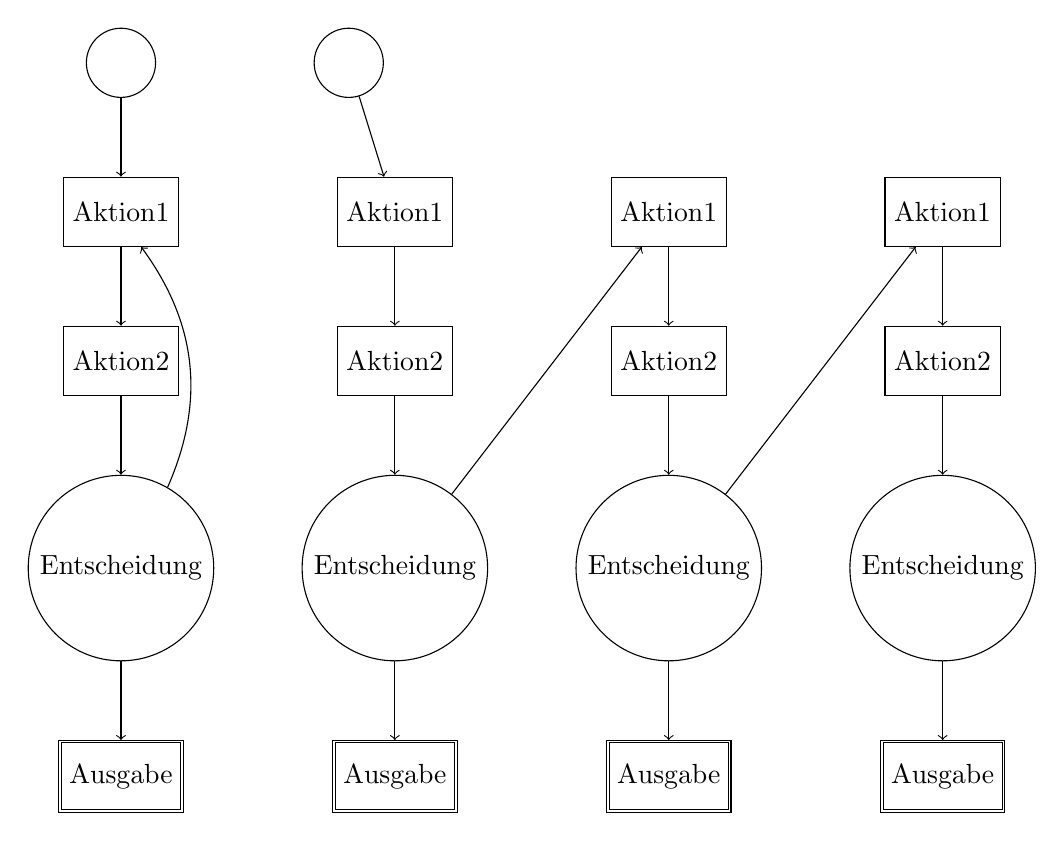
\begin{tikzpicture}[]
        %Graph links
        \node[state, initial text=""](q0){};
        \node[state, rectangle, below = 1cm of q0](q1){Aktion1};
        \node[state, rectangle, below = 1cm of q1](q2){Aktion2};
        \node[state, below = 1cm of q2](q3){Entscheidung};
        \node[state, accepting, rectangle, below = 1cm of q3](q4){Ausgabe};

        \draw(q0) edge[->] (q1);
        \draw(q1) edge[->] (q2);
        \draw(q2) edge[->] (q3);
        \draw(q3) edge[->, bend right] (q1);
        \draw(q3) edge[->] (q4);

        %Graph rechts
        \node[state, initial text="", right = 2cm of q0](q5){};
        \node[state, rectangle, right = 2cm of q1](q6){Aktion1};
        \node[state, rectangle, right = 2cm of q2](q7){Aktion2};
        \node[state, below = 1cm of q7](q8){Entscheidung};
        \node[state, rectangle, accepting, below = 1cm of q8](q9){Ausgabe};

        \node[state, rectangle, right = 2cm of q6](q10){Aktion1};
        \node[state, rectangle, right = 2cm of q7](q11){Aktion2};
        \node[state, below = 1cm of q11](q12){Entscheidung};
        \node[state, rectangle, accepting, below = 1cm of q12](q13){Ausgabe};

        \node[state, rectangle, right = 2cm of q10](q14){Aktion1};
        \node[state, rectangle, right = 2cm of q11](q15){Aktion2};
        \node[state, below = 1cm of q15](q16){Entscheidung};
        \node[state, rectangle, accepting, below = 1cm of q16](q17){Ausgabe};

        \draw(q5) edge[->] (q6);
        \draw(q6) edge[->] (q7);
        \draw(q7) edge[->] (q8);
        \draw(q8) edge[->] (q9);
        \draw(q8) edge[->] (q10);
        
        \draw(q10) edge[->] (q11);
        \draw(q11) edge[->] (q12);
        \draw(q12) edge[->] (q13);
        \draw(q12) edge[->] (q14);

        \draw(q14) edge[->] (q15);
        \draw(q15) edge[->] (q16);
        \draw(q16) edge[->] (q17);


    \end{tikzpicture}
    }
    \\\textbf{Abbildung TODO} Algorithmus Schleifenentfaltung\\
    \\Auf die Vor- und Nachteile der Implementierung wird im Kapitel~\ref{Evaluation} eingegangen.
    \subsection{2. Lösungsansatz}
    Schleife soll durch ein Konstrukt realisiert werden.
    Prüfungslogik muss um eine weitere Aktivitätsaktion erweitert werden. Das Schleifenkonstrukt greift dabei auf bereits vorhandene Regeln der Prüfungslogik zu.
    Das Schleifenkonstrukt greift dabei wie die anderen Aktivitätsaktionen auf den Referenzstack zu. Da der nächste Schleifendurchlauf nicht wieder auf den gleichen Eingabenwerten laufen soll, da diese wieder zu einem fehlerhaften Wert führen wird, muss ein Mechanismus im Schleifenkonstrukt implementiert werden, welcher einen neuen Wert holt.
    Durch die einführung der Schleife entstehen neue Herausforderungen. Es können nun Endlosschleifen entstehen, welche dazuführen dass die ausgeführte Prüfung niemals terminieren wird. Außerdem liefert der Hauptuntersuchungs-Adapter keine linearen Werte (?), sondern nicht determenistische Werte.

    Eine Endlosschleife kann von vorneherein ausgeschlossen werden, indem die maximalen Schleifendurchläufe begrenzt werden. 
    Da die Werte des Hauptuntersuchungs-Adapter nicht vorhersehbar sind und die Prüfung nicht jedes mal die maximale Anzahl der Schleifendurchläufe ausführen soll, muss ein Algorithmus entwickelt werden, welcher sagt wann man davon ausgehen kann, wann die ausgelesenen Sensorwerte sicht großartig nicht mehr ändern und stabil sind.
    
    Ein möglicher Lösungsvorschlag könnte nun folgendermaßen aussehen. 
    Je nachdem welcher Typ der Eingabewert hat verläuft der Algorithmus anders. Es wird dabei nur zwischen Zahlen und Zeichenketten unterschieden. 
    Bei Zeichenketten wird der aktuelle Wert mit dem Wert aus dem vorherigen Schleifendurchlauf verglichen. Dafür wird die Levenshtein-Distanz verwendet. Beim ersten Schleifendurchlauf wird als zweite Zeichenkette das leere Wort $\epsilon$ verwendet. $\epsilon$ wird verwendet, weil dieser Wert keinen negativen Ablauf auf den Algorithmus haben wird. Dies wird im weiteren Verlauf der Erklärung genauer erklärt. 
    Die Levenshtein-Distanz gibt die ähnlichkeit zwischen zwei Zeichenketten als Zahl an, indem sie die minimale Anzahl an Operation angibt, welche benötigt werden, damit die erste Zeichenkette der zweiten Zeichenkette gleicht. Je größer die Zahl ist destso "unterschiedlicher" sind die beiden Zeichenketten von einander. 

    Um zu schauen wie sich die Eingabe zu verschiedenen Zeiträumen verhält, berechnen wir Mittelwerte über TODO. Es sollten mindestens zwei Mittelwerte gebildet werden. Mehr als zwei Mittelwerte sind möglich, aber würden den Algorithmus entwindlicher machen. Der erste Mittelwert sollte über alle bisherigen Eingaben gebildet werden, um zu sehen wie sich die Eingabe auf langer Sicht verhält. Der zweite Mittelwert sollte über die letzten n Eingaben gebildert, um zu sehen wie sich die Eingabe auf kurzer Sicht verhält.
    Da die Werte der Levenshtein-Distanz sich für den Mittelwert nicht besonders anbieten, müssen die Zeichenketten in einen Zahlenwert umgewandelt werden.
    Das kann geschaffen werden indem alle Zeichen der Zeichenkette in eine eindeutige Zahl umwandeln und die einzelnen Zahlen anschließend Addieren. Damit wir uns um die Umwandlung keine Sorgen machen müssen, greifen wir dafür auch die ASCII-Tabelle zu.
    Zusätzlich muss eine Gewichtung bei der Addition berücksichtigt werden, weil sonst Zeichenketten, die aus den gleichen Zeichen bestehen, den gleichen Wert bei der Addition rausbekommen. Das liegt daran, dass bei der Addition ohne Gewichtung nur die Wertigkeit der einzelnen Zeichen betrachtet wird, aber nicht deren Position. Dieses Problem wird mit der Gewichtung aufgelöst. Ein Beispiel dafür für die Addition mit Gewichtung ist in Abbildung TODO.
    Dies muss aber nicht für jedes Eingabepaar gemacht werden, sondern nur für Eingabepaare welche sich sehr ähneln, also eine niedrige Levenshtein-Distanz haben. Für Eingabepaare mit einer hohen Levenshtein-Distanz ist das nicht notwendig, weil wir da bereits wissen, dass sich die Zeichketten stark von einerander unterscheiden.
    Ist die Differenz aus der umgewandelten umgewandelten Zeichenkette und einem Mittel kleiner als ein vordefinierter Schwellenwert, wissen wir dass die Zeichenkette sich nur ganz leicht von den durchschnittlichen Eingaben unterscheidet.
    Wenn dies nun mehrmals nacheinander vorkommt, kann davon ausgegangen werden, dass der Wert in diesen Wertebereich stagniert.
    Um dies im ALgortithmus auch zu berücksichtigen, wird ein n-Chance Mechanismus eingebaut der folgendermaßen Funktioniert:
    \begin{itemize}
        \item Wird der Schwellenwert unterschritten, wird unser n dekrementiert.
        \item Wird der Schwellwert übertroffen oder ist unsere Differenz gleich wird n zurückgesetzt.
        \item Erreicht n irgendwann die 0 wird die Schleife abgebrochen. 
    \end{itemize}
    %Beispiel
    $
        "foo" = 102 + 111 + 111 = 324
        "oof" = 111 + 111 + 102 = 324
        mit Gewichtung
        "foo" = 1 * 102 + 2 * 111 + 3 * 111 = 657
        "oof" = 1 * 111 + 2 * 111 + 3 * 102 = 639
    $
    \\\textbf{Abbildung TODO} Beispiel Addition mit und ohne Gewichtung
    \\\\Ist unser Eingabewert nun keine Zeichenkette, sondern eine Zahl entfällt der Umwandlungsschritt mit der Gewichtung. Es kann sofort mit den beschriebenen Mittelwertansatz angefangen werden.
    %Schleifenkonstrukt -> Benutzer gibt Abbruchbedigung ein (Benutzer verwendet Schleifenkonstrukt statt Entscheidungs Aktivität) -> 
    %typ (generisch?, damit das System dies für uns übernimmt) der eingabe muss bestimmt werden, damit richtiger algorithmus zur stabilität überprüfung ausgewählt werden kann (es wird nur zwischen zeichenketten und zahlen unterschieden => bei zahlen wird mittelwertansatz gewählt bei zeichenketten Levenshtein-Distanz)
    %Was muss geändert werden: Prüfungslogik muss durch die aktivität schleife erweitert werden
    %Schluss
    \newpage
    \section{Evaluation}
    \label{Evaluation}
    \subsection{}
    \subsubsection{1. Lösungsansatz}
    +einfach zu implementieren, da wir kein schleifenkonstrukt mehr benötigen.
    +keine Endlosschleife, weil es keine Schleifen gibt
    +keine Zyklen, weil der Ablauf linear ist
    +weniger Sprünge, weil keine for oder while Bedingungen vorhanden sind
    +möglicher Performance gewinn, weil Schleifen-Overhead entfällt
    -größerer Codeumfang, da der eigentliche schleifenkörper a-mal im code implemtniert werden muss 
    -höherer verbraucht an ressourcen zB Speicher mehr code = mehr speicher
    -möglicherweise ineffizient, wenn der faktor zu groß gewählt wird
    -schlechtere Lesbarkeit
    -wenn bereits nach 3 durchlaufen feststeht, dass das gewünschte ergbeniss nicht mehr erreicht werden kann werden trotzdem die restlichen schritte ausgeführt
    \subsection{2. Lösungsansatz}
    +keine Endlosschleife, weil maximale Schleifendurchläufe begrenzt sind.
    +
    -azyklisches verhalten wird verletzt, weil schleifenkonstrukt benötigt wird
    -
    \newpage
    \renewcommand{\refname}{}
    \section{Literaturverzeichnis}
    \begin{thebibliography}{9}
        \bibitem{2}Johnston, W., Hanna, J., \& Millar, R. (2004). \emph{Advances in dataflow programming languages}. ACM Computing Surveys, 36(1), 1–34.
        \bibitem{3}Chen, L. (2021). \emph{Iteration vs. Recursion: Two Basic Algorithm Design Methodologies}. SIGACT News, 52(1), 81–86.
        \bibitem{4}Arvind, \& Culler, D. (1986). \emph{Dataflow Architectures}. LCS Technical Memos.
        \bibitem{5}Ambler, A., \& Burnett, M. (1990). \emph{Visual forms of iteration that preserve single assignment}. Journal of Visual Languages \& Computing, 1(2), 159–181.
        \bibitem{6}Mosconi, M., \& Porta, M. (2000). \emph{Iteration constructs in data-flow visual programming languages}. Computer Languages, 26(2), 67–104.
        \bibitem{1}Fan, Z., Li, W., Liu, T., Tang, S., Wang, Z., An, X., Ye, X., \& Fan, D. (2022). \emph{A Loop Optimization Method for Dataflow Architecture}. In 2022 IEEE 24th Int Conf on High Performance Computing \& Communications; 8th Int Conf on Data Science \& Systems; 20th Int Conf on Smart City; 8th Int Conf on Dependability in Sensor, Cloud \& Big Data Systems \& Application (HPCC/DSS/SmartCity/DependSys) (pp. 202–211).
        \bibitem{7}Gévay, G., Soto, J., \& Markl, V. (2021). \emph{Handling Iterations in Distributed Dataflow Systems}. ACM Comput. Surv., 54(9), 199:1–199:38.
        \bibitem{8}Alves, T., Marzulo, L., Kundu, S., \& França, F. (2021). \emph{Concurrency Analysis in Dynamic Dataflow Graphs}. IEEE Transactions on Emerging Topics in Computing, 9(1), 44–54.
        \bibitem{9}Ye, Z., \& Jiao, J. (2024). \emph{Loop Unrolling Based on SLP and Register Pressure Awareness}. In 2024 20th International Conference on Natural Computation, Fuzzy Systems and Knowledge Discovery (ICNC-FSKD) (pp. 1–6).
        \bibitem{10}Lučanin, D., \& Fabek, I. (2011). \emph{A visual programming language for drawing and executing flowcharts}. In 2011 Proceedings of the 34th International Convention MIPRO (pp. 1679–1684).
        \bibitem{11}Davis, A., \& Keller, R. (1982). \emph{Data Flow Program Graphs}. All HMC Faculty Publications and Research.
        \bibitem{21}Boshernitsan, M., \& Downes, M. (2004). \emph{Visual Programming Languages: A Survey}. EECS University of California, Berkeley.
        \bibitem{12}Charntaweekhun, K., \& Wangsiripitak, S. (2006). \emph{Visual Programming using Flowchart}. In 2006 International Symposium on Communications and Information Technologies (pp. 1062–1065).
        \bibitem{13}Burnett, M., Baker, M., Bohus, C., Carlson, P., Yang, S., \& Van Zee, P. (1995). \emph{Scaling up visual programming languages}. Computer, 28(3), 45–54.
        \bibitem{14}Kurihara, A., Sasaki, A., Wakita, K., \& Hosobe, H. (2015). \emph{A Programming Environment for Visual Block-Based Domain-Specific Languages}. Procedia Computer Science, 62, 287–296.
        \bibitem{15}Hils, D. (1992). \emph{Visual languages and computing survey: Data flow visual programming languages}. Journal of Visual Languages \& Computing, 3(1), 69–101.
        \bibitem{19}Sousa, T. (2012). \emph{Dataflow Programming Concept, Languages and Applications}. Doctoral Symposium on Informatics Engineering, 7.
        \bibitem{18}Van Deursen, A., Klint, P., \& Visser, J. (2000). \emph{Domain-specific languages: an annotated bibliography}. ACM SIGPLAN Notices, 35(6), 26–36.
        \bibitem{16}Roy, G., Kelso, J., \& Standing, C. (1998). \emph{Towards a visual programming environment for software development}. In Proceedings. 1998 International Conference Software Engineering: Education and Practice (Cat. No.98EX220) (pp. 381–388). IEEE Comput. Soc.
        \bibitem{20}Weintrop, D. (2019). \emph{Block-based programming in computer science education}. Communications of the ACM, 62(8), 22–25.
        \bibitem{22}Gumm, H.P., \& Sommer, M. (2016). \emph{Band 1 Programmierung, Algorithmen und Datenstrukturen}. De Gruyter Oldenbourg.
    \end{thebibliography}
\end{document}    